\documentclass{article}

\usepackage[english]{babel}
\usepackage{microtype}
\usepackage{graphicx}
\usepackage{wrapfig}
\usepackage{enumitem}
\usepackage{fancyhdr}
\usepackage{amsmath}
\usepackage{chemformula}
\usepackage{index}
\usepackage{hyperref}
\usepackage[margin=1.0in]{geometry}
\usepackage{qtree}
\usepackage{float}
\usepackage{booktabs}
\usepackage{tabularx}
\usepackage{textcomp}

\begin{document}
\title{Summary: Locomotion}
\author{Dowland Aiello}
\date{April 20, 2020}

\maketitle
\tableofcontents
\fancyhf{}

\newpage

\section{Overview: Locomotion}

When an animal isn't moving, it is kept in place through two forces: gravity and
friction. When an organism overcomes these forces and moves, an organism
engages in \textbf{locomotion}, or active travel from one place to another.
Regardless of implementation details that differ between organisms, all types of
locomotion require the movement of protein strands against each other. This
behavior is demonstrated in avrious organisms and environments, such as:

\begin{itemize}
    \item \textbf{Acquatic} animals: due the density of the water encompassing their
    natural environment, these organisms need not hastily concern themselves with
    overcoming the force of gravity, but, rather, friction.
    \item \textbf{Terrestrial} animals: due to the lack of support provided by air,
    terrestrial organisms must expend energy to counter the force of gravity,
    and, additionally, friction with respect to the ground.
    \begin{itemize}
        \item Walking animals
            \begin{itemize}
                \item Bipedal animals: utilize just two limbs (legs) in
                maintaining balance, maintaining contact with the ground on at
                least one foot, but lack the stability of their quadrapedal or
                tripedal equivalents
                \item Quadrapedal animals: constantly utilize at least three feet
                in maintaining balance
                \item In both quadrapedal and bipedal animals, momentum plays
                an important part in the persistence of balance while running
            \end{itemize}
        \item Hopping animals
            \begin{itemize}
              \item Kangaroos: travel by generating power in hind leg muscles,
                and by storing energy in connected tendons
            \end{itemize}
        \item Crawling animals
            \begin{itemize}
                \item Energy expenditure is focused towards friction
                \item Snakes: entire body is undulated from side to side
                \item Earthworms: perform a sequence of muscle contractions from
                head to tail (\textbf{peristalsis})
            \end{itemize}
        \item Flying animals (i.e., birds, bats, and various invertebrates)
            \begin{itemize}
                \item Energy expenditure is focused towards combating gravity
                and developing ``lift.''
              \item Capability is reliant on airfoil-like wing structures that
                create lift, inducing an air pressure different conducive to
                flight
            \end{itemize}
    \end{itemize}
\end{itemize}

\section{Role of the Skeletal system in locomotion}

\subsection{Hydrostatic Skeletons}

The \textbf{hydrostatic skeleton} is one of the three commonly cited types of
skeletons (i.e., hydrostatic skeletons, exoskeletons, and endoskeletons), and it
consists of the pressurized enclosure of fluid in a compartment. This structure
can be differentiated widely from its external and internal counterparts, but is
commonplace in both terrestrial and aquatic animals, who each share various
similarities:

\begin{itemize}
    \item Flexibility and a soft texture
    \item Burrowing or crawling behaviors via peristalsis
\end{itemize}

Though they share similiar behaviors and generalized structures, the various
organisms that utilize this form of skeleton build upon the functional base of
a hydrostatic skeleton in unique ways. Earthworms, for example, are capable of
persitalsis by forcing circular and longitudal muscles to work ``against'' their
skeletons. Hydras and jellies, on the other hand, are capable of modifying their
body shape through the exertion of pressure.

Hydrostatic skeletons are ill-suited for terrestrial animals whose modes of
locomotion mimic that of humans (i.e., above-ground movement akin to walking).

\subsection{Differences between Exoskeletons and Endoskeletons}

The term ``invertebrate'' or ``vertebrate'' is often used to describe various
organisms. These terms are used to describe organisms with \textbf{exoskeletons}
and \textbf{endoskeletons}, respectively. The central difference with respect to
these two types of skeletons lies in the location of the skeleton: in
exoskeleton systems, the entire system lies outside of the body, while in
endoskeleton systems, the system lies inside the body. Furthermore, in contrast
to vertebrates, invertebrates are not capable of growing alongside their
skeletons, and, thus, ``shed'' or \textbf{molt} their exoskeletons at regular
intervals. By comparison, in vertebrates, skeletal systems are typically
composed
of cartilage or bone, rather than \emph{strictly} inorganic, static material,
thus mitigating a need for ``shedding'' behaviors.

\bigbreak{}

\begin{figure}[h]
  \centering
  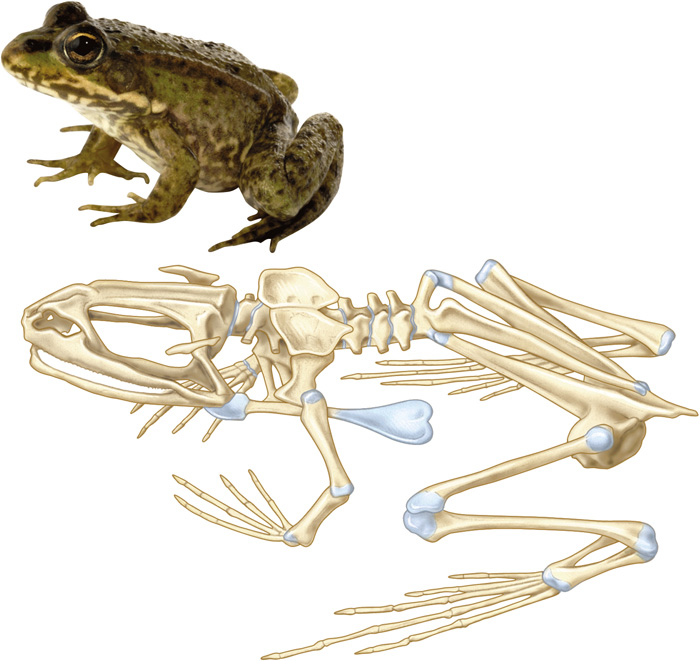
\includegraphics[width=0.7\linewidth]{frog_skeletal_system.jpg}
  \caption{The skeletal system of a frog}
\end{figure}

\subsection{Common Components of Vertebrate Skeletons}

In all vertebrates, there exist several components in a skeletal system:

\begin{itemize}
    \item An \textbf{axial skeleton}: the ``trunk'' of the body, consisting of
    the:
        \begin{itemize}
            \item Skull: protects the brain
            \item Backbone: consists of disc-conjoined vertebrae (i.e.,
            24 cartilage pade-conjoined vertebrae in humans, and 400 in
            pythons), comprising various regions of the vertebral column:
                \begin{itemize}
                    \item Cervical / neck: supports the head
                    \item Thoracic / chest: forms joints with the ribs
                    \item Lumbar / lower back
                    \item Sacral / between the hips
                    \item Cocygeal / tail
                \end{itemize}
            \item Commonly, rib cage
        \end{itemize}
  \item An \textbf{appendicular skeleton}: anchors appendages (e.g., legs and
    arms) to the axial skeleton
\end{itemize}

\subsection{The structure of a bone}

In endoskeletal systems, bones are living---that is, they are comprised by
various living tissues:

\begin{itemize}
    \item Coating fibrous connective tissue: allows for the formation of a
    newpagebone in a fracture
    \item Cushioning cartialage: protects bones as they glide past each other
    \item Various \textbf{matrix}-secreting constituent living cells
    \item \textbf{Bone matrix}: protein collagens that keep the bone flexible and
    a collection of compression-resistent minerals
    \item \textbf{Yellow bone marrow}: stored fat delivered by way of blood
    \item \textbf{Red bone marrow}: produces blood cells
\end{itemize}

\section{Functional actors in locomotion}

\subsection{Joints}

A \textbf{join} is defined as ``a point at which parts of an artificial
structure are joined.'' In endoskeletal systems, \textbf{ligaments}, fibrous
connective tissue, are utilized in various bone-connected movable joints:

\begin{itemize}
    \item \textbf{Ball-and-socket joints}: enable the rotation of arms and legs,
    and are found where the humerus joins the pectoral girdle
    \item \textbf{Hinge joints}: permit movement about a plane (e.g., elbows and
    knees)
    \item \textbf{Pivot joints}: permits side-to-side movement
\end{itemize}

\bigbreak{}

\begin{figure}[h]
    \centering
    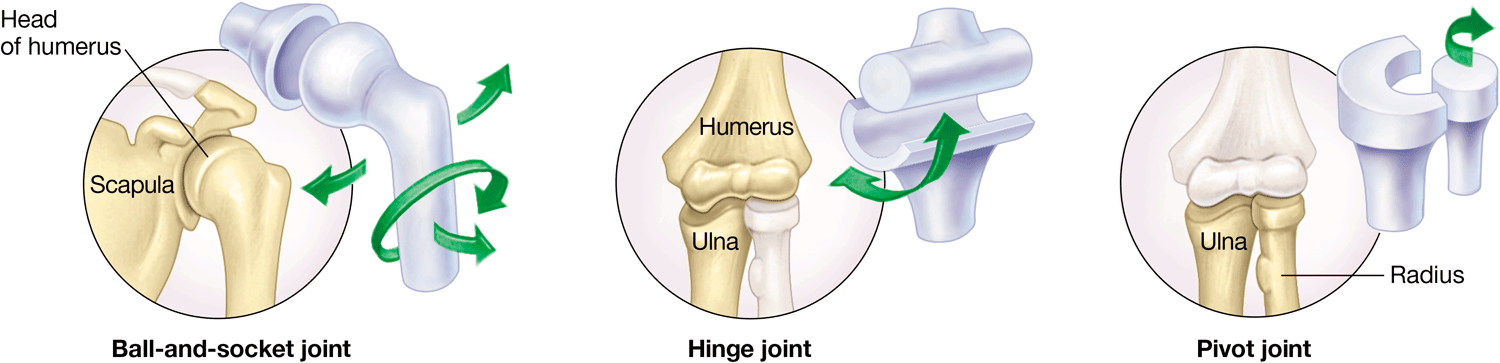
\includegraphics[width=\linewidth]{types_of_joints.png}
    \caption{The three kinds of joints}
\end{figure}

\subsection{Muscles}

\begin{wrapfigure}{r}{0.5\textwidth}
  \centering
  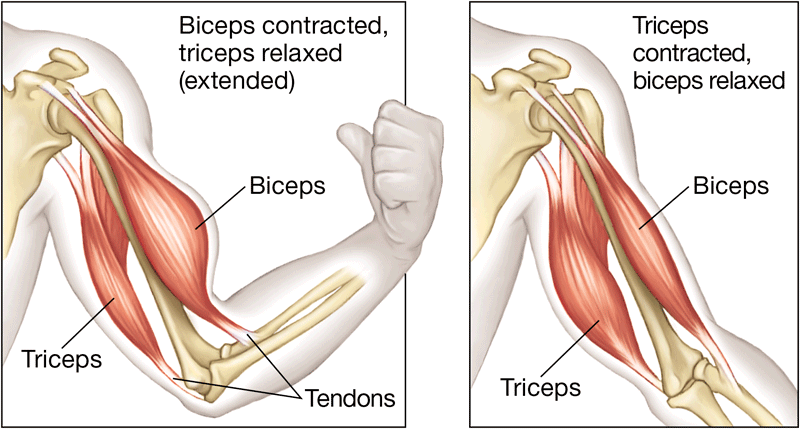
\includegraphics[width=\linewidth]{muscle_action.png}
  \caption{Antagonistic action of muscles in the human arm}
\end{wrapfigure}

Muscles aid in locomotion through their innate tendencies to contract and
normalize with respect to \textbf{tendon} connections. At these connections,
muscles are attached to bones, introducing a fixed tendency to perform these
actions, respectively.

\end{document}
